\section{Contexto histórico}

La burbuja de los Mares del Sur coincidió con el rápido desarrollo de los mercados financieros en Europa a finales del siglo XVII y principios del XVIII. Este período vivió la introducción de un mercado secundario activo tanto en deuda como en renta variable. 

Se ubica el nacimiento de la Compañía de los Mares del Sur en el año 1.711 de la mano de Robert Harley. La situación del gobierno inglés por aquel entonces no era estable y necesitaba sanear sus cuentas de un modo sencillo y rápido. Se creyó que una brillante forma de llevarlo a cabo sería poniendo en marcha el comercio con América del Sur. Este mercado consistiría en la recolecta de metales preciados y pieles entre otros productos, por los que en Europa se obtendrían grandes beneficios.

El mayor problema era que Inglaterra estaba en guerra con España y ésta poseía el control de casi todos los países suramericanos. Pero en 1.713, se dio por finalizada la Guerra de Sucesión Española, e Inglaterra pudo comenzar a comerciar con América del Sur, si bien de una forma muy limitada, hasta que en 1.718 volvieron a enfrentarse en una nueva guerra donde Inglaterra salió victoriosa. Un año más tarde, los ingleses se hicieron con parte del control del mercado con América del Sur. De este modo, la Compañía de los Mares del Sur se vio reforzada contando con barcos de esclavos y barcos textiles que navegaban bajo la bandera de la Compañía. Aun así, desde sus inicios, la Compañía estaba más involucrada en subsanar los problemas de la deuda, tema que se tratará con más detalle a lo largo del capítulo. 

\section{Surgimiento de las cofee houses}

Los comerciantes del siglo XVIII y los inversores tuvieron que depender en gran medida de las \emph{coffee houses}, es decir, las cafeterías, y también de la prensa para obtener información acerca de las inversiones y de los movimientos del mercado. Estas dos fuentes de información eran interdependientes, ya que los periodistas obtenían gran parte de sus informaciones en estas cafeterías.

Después de 1.695, los medios de comunicación comenzaron a desarrollarse proporcionando una gama cada vez más amplia de publicaciones para su clientela. Por su parte, las cafeterías en Londres proliferaron a partir del siglo XVI y en el año 1.700 había más de 2.000, convirtiéndose no sólo en un lugar de ocio, sino en una biblioteca donde las revistas podían ser estudiadas por un público ávido de noticias, lo que supuso una revolución en los hábitos sociales y de ocio de la población. La clientela inicial que frecuentaba las cafeterías, era de carácter selecto, por ejemplo casas literarias, sabios eruditos, políticos y abogados entre otros. Para llevar a cabo transacciones comerciales existían cafés especializados que atendían a las compañías marítimas y a empresas de seguros de vida.

Una de las funciones más destacables de las cafeterías es que eran una fuente muy importante de información política, económica y financiera. En efecto, antes de que existiese la libertad de prensa eran probablemente la principal fuente de noticias.

\section{La compañía de los Mares del Sur}

Hay que destacar la semejanza, que en un principio, podrían mostrar las dos situaciones financieras, tanto la de Inglaterra como la de Francia. Al desarrollarse en primer lugar la de la Compañía del Mississippi, es inevitable destacar la influencia de la teoría del dinero y el sistema desarrollado por John Law. El gobierno inglés se percató de que atravesaban una situación similar a la francesa, es decir, se estaban buscando alternativas a la resolución de su deuda pendiente acumulada, y su planteamiento era un esquema similar a la operación del Mississippi que llevó a cabo Law. 

Por otro lado, el primer director de la compañía compró deuda estatal en el año 1.719. Emitiendo así, acciones por las que se recibían dividendos todos los años. De este modo, Inglaterra lograba obtener liquidez para saldar deudas. 

Tras un proceso de licitación entre el Banco de Inglaterra y la Compañía de los Mares del Sur, esta última ganó el derecho a comprar 31,5 millones de libras en anualidades del Estado a largo plazo, a corto, e incluso deudas reembolsables. Las anualidades son ingresos periódicos de los que goza el comprador de la acción, bien a corto plazo o a largo plazo. En cambio, en las deudas reembolsables, la deuda es amortizable cuando en un momento determinado hay que pagar íntegro el capital. 

El gobierno accedió a adquirir el crédito de la Compañía ya que eso suponía un incremento en el presupuesto estatal de 31,5 millones de libras esterlinas. Así, ese nuevo capital se podía emplear para pagar las deudas adquiridas por el Estado. 

\section{Evolución de la burbuja económica de los Mares del Sur}

Algunos estudios han enmarcado a esta burbuja como un comportamiento irracional basándose en gran medida en anécdotas y citas contemporáneas. Contribuciones más recientes han tratado de explicar el aumento de la cotización de las acciones de la Compañía de los Mares del Sur en un marco racional.

Se ha de tener en cuenta, que los datos empleados en los últimos años, a la hora de analizar la burbuja de los Mares del Sur, nunca se habían tenido en cuenta en los estudios de la época. Los resultados ponen de manifiesto la falta de relación de los contratos a largo plazo y los precios se suscripción de las acciones de la compañía de los Mares del Sur.

Sin embargo, estos resultados dependen fundamentalmente de las fuentes de donde se colecten los precios de las acciones, los precios de suscripción y el tipo de interés al que los bancos prestaban dinero. Éstos, deben ser lo más fiables posible.

En contraposición, Garber (2.000) llega a la conclusión de que la burbuja de los Mares del Sur se puede comprender como un caso de especulación en la que los inversores trabajan sobre la base de los mejores análisis económicos disponibles y los precios empujan hacia el incremento a lo largo de su camino. Esto se debe a su visión cambiante de los fundamentos del mercado. Por esta razón, defiende la inexistencia de burbuja económica en la Compañía de los Mares del Sur.

\subsection{Tipos de contratos y análisis de precios}

Para realizar un correcto análisis, hay que recordar que las suscripciones son opciones sobre acciones que para mantener viva la opción, el suscriptor tuvo que realizar pagos periódicos. Por lo que se deduce que las acciones no se entregan inmediatamente. Por consiguiente, la fecha de liquidación era indefinida y el contrato con los suscriptores seguía vigente pero las entregas de las acciones todavía no se hacían efectivas. En consecuencia, había dos tipos de contrato en los abonos: 

\begin{enumerate}
	\item \emph{Mercado secundario}: Se trata de adquisiciones de acciones que ya han sido emitidas anteriormente en el mercado.
	\item \emph{Contratos forward}: Donde los compradores pagan por adelantado al precio actual de mercado con la previsión de contar con las acciones en un momento futuro determinado.
\end{enumerate}

Teniendo en cuenta estos contratos, se va a proceder a realizar un análisis de precios sustentado por autores relevantes.

En primer lugar, John Freke (1720), autor de la época, publica diferentes precios para las dos clases de contratos, es decir, para los contratos forward y para los contratos en mercados secundarios para la tercera y cuarta suscripción. 
En segundo lugar, según indica Freke, si en algún momento existe divergencia de precios entre los dos tipos de contratos, siempre usará como referencia el contrato forward.

Los estudios de Neal (2.009) dan una opinión acerca de la crisis de la Compañía de los Mares del Sur. Para este autor, no es más que una crisis crediticia que ocurrió en plena burbuja económica. Hay evidencia de que el Banco de Inglaterra prestaba líquido al 5 por ciento a lo largo de todo el período cubierto por el análisis, pese a que se llevan a cabo criterios más estrictos para los préstamos en las últimas etapas de la burbuja. 

Hutcheson (1.720), señala que algunos individuos estaban pagando tasas muy altas ya en abril de 1.720. Aun así, debieron ser más cuidadosos ya que se otorgaron préstamos a individuos sin capacidad crediticia lo que provocó que se asumiese un alto riesgo de incumplimiento de pagos. 

En resumen, la evidencia sugiere que el 5 por ciento es una tasa de descuento apropiada para el período en el que la burbuja perduró. 

Al analizar las cuatro suscripciones de dinero de una manera equitativa, el resultado es que ninguna sufre desventaja, ya que cada suscripción se limitó a presentarse como un medio para adquirir liquidez a través de un sistema de pagos escalonados, que varían para cada suscripción. Una vez descontados adecuadamente los pagos a plazos de las cuatro suscripciones, los valores y las suscripciones de acciones se convierten en instrumentos directamente sustituibles entre sí, ya que representan activos equivalentes y dividendos. En consecuencia, los precios de suscripción ajustados se pueden comparar directamente entre sí y también con el precio de las acciones. 

\begin{table}
\begin{tabular}{llllllll}
\hline
\multicolumn{2}{c}{\emph{Primera suscripción}} & \multicolumn{2}{c}{\emph{Segunda subscripción}} & \multicolumn{2}{c}{\emph{Tercera subscripción}} & \multicolumn{2}{c}{\emph{Cuarta subscripción}}
\tabularnewline
\multicolumn{2}{c}{\emph{(Libras)}} & \multicolumn{2}{c}{\emph{(Libras)}} & \multicolumn{2}{c}{\emph{(Libras)}} & \multicolumn{2}{c}{\emph{(Libras)}}\tabularnewline
\hline 

 14 abril   & 60 & (29 abril) & 40              & 16 junio & 100 & 24 ago. & 200 \tabularnewline
 1720 &     & 1720            &                 & 1720 &   & 1720 &   \tabularnewline
 14 junio   & 30              & 14 sept.        & 40 & 2 enero & 100 & 24 sept. & 200 \tabularnewline
            &                 & (24 ago.)       &   & 1721 & 100 & 1721 &   \tabularnewline
 14 agosto  & 30              & 14 ene. 1721    & 40 & 2 julio & 100 & 24 agosto & 200 \tabularnewline
            &                 & (24 dic.)       & 40 &   & 100 &   & 200 \tabularnewline
 14 octubre & 30              & 14 mayo         & 40 & 2 enero & 100 & 24 febr. & 200 \tabularnewline
            & 30              & (24 abril)      & 40 & 1722 & 100 & 1722 & 200 \tabularnewline
 14 febrero & 30              & 14 sept.        & 40 & 2 julio & 100 & 24 agosto & 200 \tabularnewline
 1721       &                 & (24 ago.)       & 40 & 2 julio & 100 & 24 agosto & 200 \tabularnewline
 14 abril   & 30              & 14 dic.         & 40 & 2 enero & 100 &   &   \tabularnewline
   &        & (24 dic.)       &                 & 1723  &   &   &   \tabularnewline
 14 junio   & 30              & 14 mar. 1722    & 40 & 2 julio & 100 &   &   \tabularnewline
            &                 & (24 abr.)       &   &   &   &   &   \tabularnewline
 14 agosto  & 30              & 14 junio        & 40 & 2 enero & 100 &   &   \tabularnewline
            &                 & (24 agosto)     &   & 1724 &   &   &   \tabularnewline
            &                 & 14 sept.        & 40 & 2 julio & 100 &   &   \tabularnewline
            &                 & (24 dic.)       &   &   &   &   &   \tabularnewline
            &                 & 14 dic.         & 40 & 2 enero & 100 &   &   \tabularnewline
            &                 & (24 abril) 1723 &   & 1725 &   &   &   \tabularnewline 
 \hline
\multicolumn{1}{r}{Total} & 300 & \multicolumn{1}{r}{Total} & 300 & \multicolumn{1}{r}{Total} & 1.000 & \multicolumn{1}{r}{Total} & 1.000 \tabularnewline 
\hline 
\tabularnewline
\end{tabular}

	\center
	\footnotesize
	Fuente: Charles Kindleberger (1.996)
	
\caption{Esquema de pagos para las suscripciones del Mar del Sur}
\label{tab:pagosSuscripciones}
	
\end{table}



Los datos de precios utilizados en el Cuadro \ref{tab:pagosSuscripciones} para la suscripción de acciones de la Compañía de los Mares del Sur es del autor John Freke (1720).  Desde 1.714 hasta 1.722 redactó y publicó dos veces por semana una lista de precios de dicha Compañía. Cada publicación abarca tres días de negociación, es decir, de miércoles a viernes, y de sábado a martes\footnote{Se debe tener en cuenta que no hay comercio los domingos.}. Freke, se encargaba de recoger los precios dados a lo largo de la mañana hasta las 15:00 horas de cada día. En ocasiones, incluye hasta tres precios por día, cuando este caso se produce se realiza un promedio simple que proporciona un único precio para el día. 

Pese a que John Freke era conocido como un defensor de la Compañía de los Mares del Sur y su plan financiero, este hecho por sí solo, no debería ser suficiente para descartar su listado de precios, porque no se puede determinar si éstos sufrieron una distorsión sistemática o si este posible hecho podría haber favorecido a la Compañía. Freke actuaba como proveedor comercial de datos, por lo que era muy consciente de que cualquier percepción distorsionada de datos destruiría su negocio. 

Otra fuente de datos alternativa es la de Castaing (1.720) y su publicación \emph{El Curso de la Bolsa}, que comenzó a divulgarse en 1.697 y que poco a poco se convirtió en la lista oficial de precios de acciones de la Bolsa.

Sin embargo, la lista de precios de Freke se emplea más a menudo porque es más completa y representa una mejor fuente a la hora de proporcionar los mejores datos en una comparación detallada durante la burbuja de la Compañía de los Mares del Sur. Por ejemplo, los precios de suscripción que expresa Freke, no son cubiertos por Castaing, sobre todo en la tercera y cuarta suscripción. 

Ambos autores se encontraban en estrecha competencia. Aunque hay que matizar que la publicación de los informes de Freke, estaba dirigida al público londinense y en cambio el estudio de Castaing puede tener destinatarios diferentes, como pueden ser individuos no residentes de Londres, que tendrían un acceso más fácil al mercado de los recibos de suscripción.  Freke, y no Castaing, hace una distinción entre el \emph{precio actual} y los precios futuros de suscripción. Esto permite hacer una comparativa más directa de los precios de las acciones y la suscripción durante el período a estudiar. 

La serie más completa de los precios de Freke se encuentra en la Biblioteca Británica, aunque faltan los datos que abarcan desde el 21 hasta el 23 de mayo de 1.720. La lista completa de datos se maneja para proporcionar una serie continuada de los precios de las acciones de la Compañía y los precios de suscripción. Dichos datos comprenden el intervalo temporal del 14 de mayo de 1.720 al 27 de septiembre del mismo año, momento en el que la burbuja comenzó a deshincharse. En cambio, los precios de suscripción están completos hasta finales de 1.720, pero su valor para este estudio es cuestionable. Esto se debe a que a finales de septiembre, la Compañía de los Mares del Sur comenzó a estudiar medidas correctoras que implicaban el ajuste retroactivo de los dos últimos precios de suscripción. 

A continuación se van a mostrar dos gráficos. En el primero de ellos, que se corresponde a la Figura \ref{fig:precioSuscripciones}, se puede observar la serie de valores y los precios de suscripción para el período desde el 14 de septiembre hasta el 27 de septiembre del año 1.720

\begin{figure}[h!]
	\caption{Precio que alcanzaron las acciones en las suscripciones en el año 1720}
	\centering
	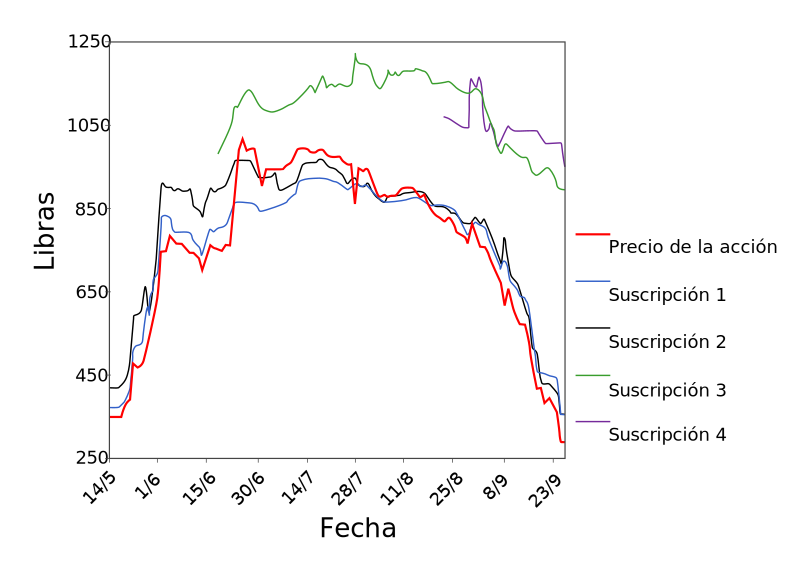
\includegraphics[width=150mm]{capitulos/graficos/precioSuscripciones}
	\label{fig:precioSuscripciones} 
	
	\footnotesize
	Fuente: Richard S. Dale, Johnnie E. Johnson \& Leilei Tang. (2.005)
	
	\raggedright
	\vspace{3 mm}
	Nota 1: Se ha utilizado la recopilación de datos de la Biblioteca británica que recogió Freke. Se ha de advertir que Freke no proporciona los precios de la suscripción número tres, es decir, del 18 a 21 junio. Por lo que los precios se han tomado son los de John Castaing. 
	
	\vspace{3 mm}
	Nota 2: Los días no comerciales, como los domingos, no se incluyen en el eje de fecha

\end{figure}

Según indican los autores de la Figura \ref{fig:tasaDeDescuento} Dale, Johnson y Tang, se puede apreciar el comportamiento irracional de la burbuja de los Mares del Sur. Esto es posible gracias a un índice que mide las tasas de descuentos que se dieron a lo largo de las cuatro suscripciones. Según el blog Gerencie, la tasa de descuento \emph{se utiliza para calcular el valor presente de los flujos de efectivo que se van a tener en el futuro; es decir los rendimientos que se esperan después de haber realizado la inversión}\footnote{Recuperado de Neira, N. (2008).}. De este modo, se puede establecer que la tasa de descuento debe corresponderse con la tasa de rendimiento requerida para los flujos de efectivo\footnote{ Según el Consejo Técnico de la Contaduría, se entiende que el flujo de efectivo \emph{es un estado financiero básico que muestra el efectivo generado y utilizado en las actividades de operación, inversión y financiación. Para el efecto debe determinarse el cambio en las diferentes partidas del balance general que inciden en el efectivo}. } que son los que determinan la capacidad de la empresa para generar efectivo. Es decir, con ella se determina el grado de cumplimiento de sus obligaciones y de sus proyectos de inversión y expansión que están asociados con la adquisición o inversión. Los factores mas importantes que hay que tener en cuenta a la hora de determinar esta tasa son: el tiempo, el mercado donde opera la empresa - en el caso que concierne a este capítulo, Compañía -, la situación política y económica del país y el sector bancario.

\begin{figure}[h!]
	\caption{Tipo de interés para los préstamos en las suscripciones}
	\centering
	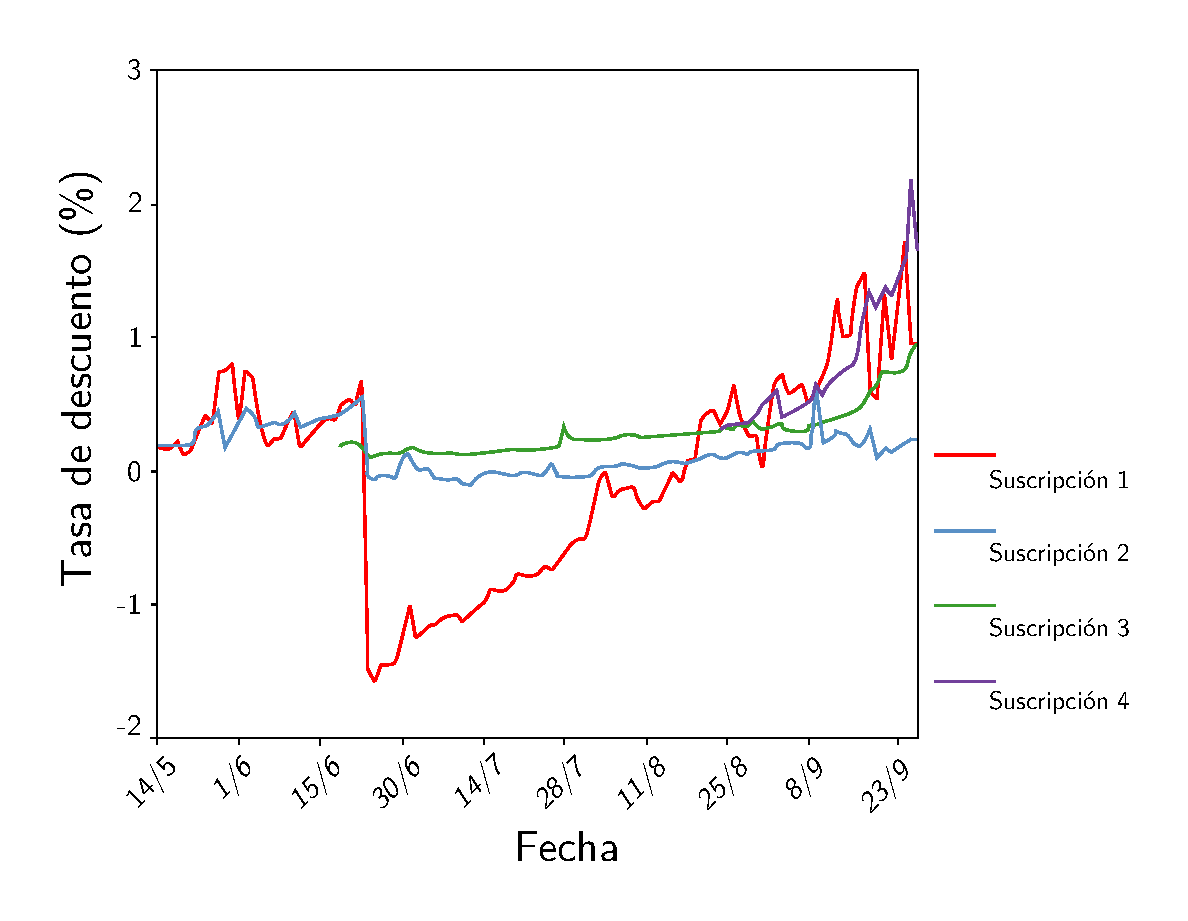
\includegraphics[width=150mm]{capitulos/graficos/tasaDeDescuento}
	\label{fig:tasaDeDescuento}

	\footnotesize
	Fuente: Richard S. Dale, Johnnie E. Johnson \& Leilei Tang. (2.005)

\end{figure}

\section{Evolución de los precios de las acciones y de las suscripciones}

La Compañía de los Mares del Sur se negó a fijar por adelantado el importe nominal de los valores canjeables\footnote{Según el blog Gerencie, los valores canjeables son \emph{los valores que pueden ser intercambiados por acciones ya existentes. No provoca ni la elevación del capital ni la reducción de las acciones}} por deuda. Cualquier aumento en el precio de la acción por encima del valor nominal provocaría una reducción de la cantidad necesaria para convertir la deuda pública pendiente. Por ejemplo, si el precio de la acción fuese 300 libras, la deuda pública de 31,5 millones de libras, podría ser comprada por la emisión de sólo 10.5 millones de libras en acciones. Los restantes 21 millones de libras de acciones emitidas, proporcionarían un posible flujo de efectivo de 63 millones de libras con el precio de mercado. 

No se dio salida al capital adicional recaudado en la emisión de acciones de la Compañía de los Mares del Sur. Este hecho, junto con el deseo de los accionistas de la Compañía de los Mares del Sur para conseguir ganancias de capital con su propia cartera de acciones, dio a la empresa un incentivo para lograr una apreciación sobre el precio de las acciones. Sin embargo, dicha valoración en el precio de la acción, proporcionó a la Compañía los medios para hacer que los dividendos se incrementasen. 

Además, se supo más tarde que en el intento por lograr la aprobación del Parlamento, la Compañía había propuesto \emph{opciones de compra}\footnote{O sobornos} a los ministros clave del gobierno y también a individuos influyentes que se encontraban estrechamente relacionados con la Corona. Este hecho proporcionó la seguridad necesaria a la Compañía a la hora de dar un impulso al precio de la acción.

A la hora de aplicar el sistema de conversión de la deuda, un escéptico miembro del Parlamento en ese periodo, lo describió como \emph{la gestión artística del espíritu del juego}. Una serie de estrategias fueron puestas en marcha para emitir más acciones, al tiempo que se maximizaba el precio de la acción de la Compañía:

\begin{enumerate}
	\item Cuatro emisiones de acciones sucesivas se ofertaron sobre los términos de suscripción generosos que implicaban tan sólo unos pequeños pagos iniciales.
	\item El guión fue diseñado para que la Compañía se mantuviese popular entre el círculo de los especuladores.
	\item Para aumentar la liquidez de los inversores y en consecuencia fomentar aún más la demanda de sus acciones, la Compañía de los Mares del Sur invitaba a los inversionistas a pedir prestado a la propia Compañía con la seguridad de que recibirían las acciones en el futuro. Más de 11 millones de libras fueron recaudadas de este modo.
	\item La Compañía de los Mares del Sur apoyó las subidas del precio de la acción mediante la compra de sus propias acciones.
	\item La compañía elevó las expectativas de los inversores, orquestando cuidadosamente los anuncios de importantes dividendos. Por ejemplo, en la víspera de la primera suscripción de dinero, que se produjo a mediados del verano, el beneficio por dividendo aumentó de un 3 por ciento a un 10 por ciento.
	\item La compañía tuvo que retrasar la emisión de acciones debido a que éstas se habían convertido en un motivo de rentabilidad. Así, no se pudo emitir recibos para la tercera y la cuarta suscripción. La intención de los directivos de la Compañía era hacer una ampliación de capital liberada \footnote{Según el centro de estudios financieros, se entiende la ampliación de capital social de una empresa como: \emph{La aportación de nuevos fondos a la sociedad, o bien de la capitalización de reservas. También puede se puede realizar una transformación de reservas a capital. Esto es posible mediante las ampliaciones de capital liberadas, en cuyo caso no se produce una entrada efectiva de fondos en la sociedad, si no que se trata de un mero apunte contable entre reservas y capital}.}y parcialmente pagada.
\end{enumerate}

Sin embargo, esta última estratagema era a lo sumo un éxito parcial, ya que los inversores podían suscribirse con total normalidad. Existen evidencias de que dichas negociaciones fueron llevadas a cabo finalmente. 

En este contexto, se puede ratificar que el precio de las acciones de la Compañía de los Mares del Sur, había avanzado desde las 130 libras en febrero de 1.720 hasta las 300 libras a principios de abril. Aun así, se continuó en esta línea de crecimiento, ya que en tan sólo once días sufrieron un incremento de doscientas libras. El 20 de mayo, el precio se situaba en 400 libras, el 28 de mayo alcanzó las 500 libras y se cerró el mes en 600 libras. Este ascenso gradual continuó el mes siguiente: el 1 de junio la acción se situaba en 700 libras y en tan sólo cuatro días aumentó cien libras alcanzando el valor de 800 libras por acción.

El 23 de junio, la empresa cerró sus libros contables durante dos meses con el fin de procesar debidamente todos los dividendos, por lo que los precios cotizados durante estos dos meses son los precios de contratos forward. Este tipo de contrato, es el más antiguo y se conoce también como \emph{contratos a plazo}. Esta clase de contrato obliga a sus participantes a comprar o vender un determinado activo en una fecha específica futura a un cierto precio\footnote{Recuperado de Zorrilla, J. P. (2010).}.

A la hora de realizar la apertura de los libros, el precio forward más alto registrado era de 1.050 libras del 25 de junio, pero cuando se reabrieron los libros, el precio al contado cayó a 820 libras. Así, la Compañía se encontró con que muchos de los que antes apoyaban sus estrategias, ahora pasaban a ser enemigos. Un claro ejemplo son los parlamentarios que exigieron la venta de parte de sus acciones al banco de Inglaterra. Aun así, el Parlamento perdonó una deuda de 7,1 millones de libras. 
Tras este desaire, el precio de las acciones de la Compañía de los Mares del Sur se debilitó drásticamente hasta descender a las 520 libras por acción, a mediados de septiembre y a 290 a principios de octubre. El mínimo se marcó el 14 de octubre de 1.720, día en que la burbuja estalló. 

\section{El banco de Hoare}
Para realizar un análisis acerca de la especulación producida a lo largo de la burbuja de los Mares del Sur, es interesante aportar un ejemplo de comportamiento comercial de un inversor sofisticado.

Este epígrafe va a dar una visión sobre las operaciones diarias de un banco propiedad de un orfebre, el Banco de Hoare. Aportando un punto de vista alternativo de cómo se puede inflar una burbuja económica a través de los registros efectuados por el propio banco. Estos datos proporcionan información sobre el tamaño del comercio, la frecuencia, el precio de ejecución, las pérdidas y ganancias, así como las órdenes que los clientes ejecutaron. 

\subsection{Historia del banco de Hoare}

El Banco Hoare era, y hoy en día continua siendo, un banco privado propiedad de la familia Hoare. Su fundador, Richard Hoare comenzó como un orfebre que trasladó su residencia en 1.690 a Londres, más concretamente a Fleet Street, donde poco después comenzó a concentrarse en la banca. El banco contaba con una larga lista de clientes de sangre azul. Entre los servicios ofrecidos por éste se encontraban los servicios de pago, los préstamos e inversión en carteras de valores, etc. También, negociaban activamente por su propia cuenta como si de autónomos se tratase. Los primeros libros de contabilidad datan de 1.702.

Desde la creación de la Compañía de los Mares del Sur, este banco invirtió en acciones de otras compañías como la \emph{Sociedad Real de África}, la \emph{Compañía de las Indias Orientales}, y el Banco de Inglaterra, así como las diversas la deudas públicas como se puede observar en el Cuadro \ref{tab:cuentaHoare}:

\begin{table}
    \begin{tabular}{lccccc}
                           & Número de        & Valor & Promedio      & Valor total & Inversión \\
                           & transacciones    & medio & de acciones   & en el       & máxima    \\
                           & en 1720          &       & en el mercado & mercado     &           \\ 
    \cline{2-6}
    Banco de Inglaterra    & 20               & 2.357 & 1.45          & 47.155      & 22.623    \\
    Compañía de las Indias & 7                & 3.423 & 1.071         & 23.96       & 14.990    \\
    Compañía de los        & 54               & 2.593 & 1.157         & 140.029     & 37.520    \\
    Mares del Sur          &                  &       &               &             &           \\
    \hline
    \end{tabular}
    
	\center
	\footnotesize
	Fuente: Charles Kindleberger (1.996)
	
    \caption {Actividad de mercado en la cuenta de Hoare en 1720}
	\label{tab:cuentaHoare}
\end{table}


La entidad financiera tuvo un éxito poco usual en su mercado. Según el estudio de Carswell (1.993), el beneficio en unidades monetarias reales ascendería a 7,1 millones de dólares. Mientras tanto, muchos inversores, algunos tan conocidos cómo Isaac Newton, perdieron importantes sumas de dinero en 1.720 debido a la burbuja económica. 

\subsection{Modelo simplificado del banco de Hoare}

Los autores Peter Temin y Hans-Joachim Voth (2.003), sostienen que en este episodio, el comportamiento de un inversor individual y su sabiduría, pueden decir mucho sobre la naturaleza de las burbujas y sobre el comportamiento de los inversores durante los periodos en los que surge una manipulación de precios. 

Tres puntos de vista a tener en cuenta debida su importancia son:

\begin{enumerate}
	\item El banco Hoare, no apostaba en contra del rápido crecimiento de la Compañía de los Mares del Sur, pero creaba indicios para que la población creyese que las acciones estaban sobrevaloradas.
	\item Era muy rentable para los participantes del mercado, ya que obtenían información de primera mano al unirse a la burbuja por un período prolongado antes de que se colapsase, en lugar de abandonar el mercado.
	\item No hay evidencias de que el banco Hoare invirtiese el dinero suficiente para comprometer la solvencia de éste. De acuerdo con el estudio teórico reciente de Abreu y Brunnermeier (2.003), parece que la necesidad de coordinación, para que la burbuja de los Mares del Sur se colapsase, fue la clave para permitir que ésta se inflase hasta el estallido. Además, el hecho de que los comerciantes racionales no lograsen evitar una burbuja era en realidad un síntoma de rentabilidad para ellos, como se refleja en los altos rendimientos obtenidos por Hoare en 1.720.
\end{enumerate}

A continuación, se va a presentar un ejemplo simplificado acerca del funcionamiento de este banco. Al ser un modelo tan abreviado no se ha de esperar dar respuesta a la totalidad de las preguntas sobre el funcionamiento de esta burbuja en concreto, pero puede arrojar luz sobre algunas de las cuestiones más importantes.

En 1.720, el banco negociaba de manera activa acciones de la Compañía de los Mares del Sur llevando a cabo cincuenta y cuatro transacciones y diecinueve operaciones destinadas a los clientes en ese mismo año. Sin embargo, tuvo su actividad máxima en las operaciones bursátiles de la Compañía. El banco, sigue un sistema de contabilidad doble y conserva un detallado registro de sus transacciones. Al igual que ocurre con las operaciones de crédito de los clientes. También se registraron las tasas de transferencia del costo total de las negociaciones. Las transacciones de los clientes abarcan los valores prestados contra la cantidad de acciones ofrecidas en garantía, la fecha de vencimiento y los intereses percibidos. 

En consecuencia, algunas de las operaciones que no estaban registradas en los libros de contabilidad, se llevaron a cabo en forma de recibos de contratos a plazos o suscripciones. En cuanto al comercio, éste fue eficiente la mayor parte del tiempo, cosa que benefició a todos aquellos en posesión de acciones o documentos de propiedad. Sin embargo, los suscriptores a menudo tuvieron que luchar con los procedimientos burocráticos diseñados para evitar una nueva suscripción de acciones. Solución que al parecer era mucho menos eficiente y eficaz que el comercio en sí. 

Los datos diarios y las pruebas fiables extremadamente detalladas de la posición del banco de Hoare, ayudan a obtener datos exactos para examinar el historial de operaciones del banco, y evaluar así, su rendimiento en comparación con el mercado y poder poner a prueba algunas hipótesis sobre el origen de su éxito. 

Para distinguir los diferentes argumentos sobre el auge de la burbuja de la Compañía de los Mares del Sur y del banco de Hoare, se describen tres situaciones que podía aportar a un inversionista en aquella época:

 \begin{enumerate}
\item Que el individuo fuese víctima de los impulsos irracionales y no de un análisis de mercado razonable. Por lo que los beneficios corrían a cargo de la suerte.
\item Que el comercio durante el tiempo en que tuvo lugar la burbuja se viese limitado por la seguridad del mercado. 
\item Que éste inversor actuase racionalmente, pero de un modo en el que favoreciese el desarrollo de la burbuja económica, es decir, comprando y vendiendo según el comportamiento esperado por los otros compradores y vendedores, es decir, siguiendo un comportamiento de \emph{herding}.
 \end{enumerate}

\subsection{El éxito del banco de Hoare}
\begin{figure}[h!]
	\caption{Comparativa del precio de las acciones de la compañía de los Mares del Sur y el mercado del banco de Hoare}
	\centering
	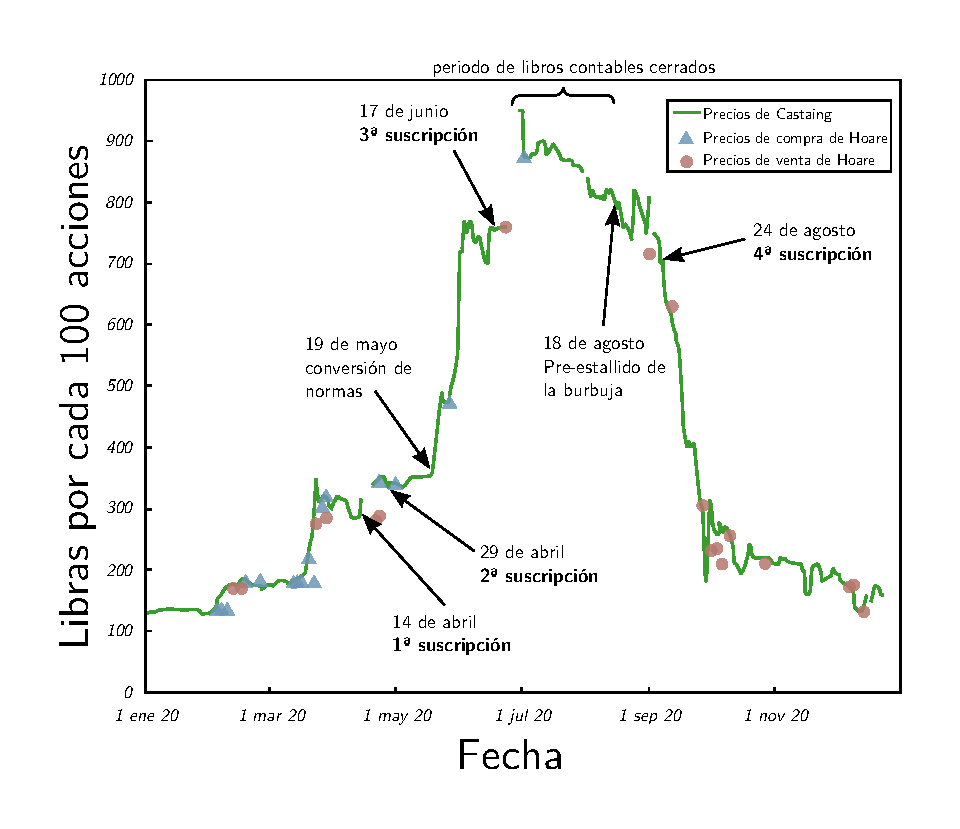
\includegraphics[width=150mm]{capitulos/graficos/bancoHoare}
	\label{fig:bancoHoare}

	\footnotesize
	Fuente: Peter Temin, \& Hans-Joachim Voth. (2.003)

\end{figure}

Como se puede comprobar en ella Figura \ref{fig:bancoHoare}, el Registro comercial de Hoare es sorprendente desde cualquier punto de vista, y este hecho no se debe al azar. Para demostrar que Hoare participó en la alimentación de la burbuja, también se ha de aclarar que el propio banco no se aprovechó de la ventaja del conocimiento de que las acciones de la Compañía de los Mares del Sur estaban sobrevaloradas. Obtener información privilegiada era sencillo ya que dentro de la larga lista de clientes del banco, muchos de ellos tenían buenos contactos que podrían haber proporcionado valiosa información.

Los clientes de Hoare que se sumergieron en el mercado durante este período fueron cruciales. En marzo de 1.720, \emph{Lord Carlton}, miembro del Parlamento, compró 6.000 acciones de la Compañía de los Mares del Sur que equivaldría a 9.000 libras que quedaron depositadas en el banco de Hoare. Éste último, a su vez había comprado 1.000 acciones el día anterior y otras 1.000 la semana anterior. A principios de marzo, pocos días antes de la transacción de Lord Carlton, el banco compró otras 7.000 acciones. Este hecho no sugiere que el banco estuviese acatando órdenes estipuladas por la Compañía de los Mares del Sur. La compra de Lord Carlton probablemente no era lo suficientemente potente como para que, sin ayuda externa, se lograse cambiar el precio de las acciones de la compañía de los Mares del Sur. Además, se ha de tener en cuenta que las compras especulativas en la Compañía de los Mares del Sur, antes del 17 de marzo, fueron muy comunes. El banco no llevó a cabo ninguna compra anterior al 21 de marzo, por lo tanto pagó el precio estipulado del 22 de marzo sobre 7000 acciones.

También hay algunas conexiones directas entre los clientes de Hoare y el pequeño grupo de iniciados que crearon la Compañía de los Mares del Sur. Sin embargo, ya que sólo se observa una información parcial a disposición de los comerciantes de la época, puede caber la posibilidad de que el éxito de Hoare derivase de que sus clientes conseguían una información privilegiada que les favorecía económicamente. 

El banco actúa normalmente como intermediario entre sus clientes y las compañías. En el caso del banco de Hoare, podía haberse beneficiado indirectamente de la certeza de que sus clientes eran conscientes de los hechos que se estaban sucediendo y de las decisiones que claramente iban a afectar al valor de las acciones. Los autores Gennotte y Leland (1.990), demuestran que, en condiciones generales, los participantes del mercado que siguen a las masas de individuos, tienden a actuar como inversores desinformados. Esto quiere decir que, compran cuando los precios descienden, y se venden cuando aumentan. Una vez que éstos reciben información precisa, por ejemplo mediante la observación de movimientos de las acciones de los inversionistas experimentados o por tener acceso a otra clase de información, sus decisiones sobre operaciones de liquidez comenzarán a tomar otro camino. En cuanto a las compras de acciones de la Compañía de los Mares del Sur, el comercio era similar. 

La combinación de los siguientes factores fue la clave el éxito del banco de Hoare. En primer lugar, la estrategia comercial por la que apostaron se basaba en la predicción de confianza de los inversores hacia las acciones durante la burbuja, apostando a que los precios subirían por un tiempo. En segundo lugar, el escenario en el que la burbuja de los Mares del Sur se desenvolvió. Es difícil distinguir entre el riesgo del comerciante y el \emph{riesgo de sincronización} de varios comerciantes. El riesgo de sincronización viene definido como \emph{la estrategia a la hora de realizar decisiones de compra o venta de activos financieros al tratar de predecir los movimientos futuros de los precios de mercado. La predicción puede basarse en una perspectiva de las condiciones del mercado o económicas resultantes de un análisis técnico o fundamental. Se trata de una estrategia de inversión basada en las perspectivas de un mercado global, en lugar de para un determinado activo financiero}. ¿Cómo se puede reducir este riesgo de sincronización? Primero se ha de analizar la actividad del inversor en busca de negociación excesiva. Y en segundo lugar, se debe emplear personal para examinar de modo selectivo y constante la actividad comercial reciente. Esta última, con el fin de identificar aquellas actitudes que puedan ser contrarias a esta política de negociación sobre sincronización con el mercado.

Según los autores Peter Temin y Hans-Joachim Voth (2.003), éstos establecen cuatro conclusiones cómo consecuencia del comportamiento comercial del banco:

\begin{enumerate}
	\item El banco de Hoare era consciente de que existían inversores sin experiencia que se encontraban mezclados con los inversores especialistas. Según los datos del banco, los que dominaron la especulación son los inversores sin experiencia. Sin embargo, parecía rentable para la propia entidad mantuviese a estos inversores en el mercado.
	\item Las restricciones de venta de acciones a corto plazo, no influyeron de manera determinante en el desarrollo de la burbuja, puesto que el banco era propiedad exclusiva de los socios. Pero si fueron un problema los incentivos surgidos de las relaciones principales de los inversores con el banco. 
	\item Según la ficha comercial de precios por parte del banco, es poco probable que fuese impulsado por el conocimiento de información privilegiada por parte de sus clientes, y como consecuencia, afectase al comportamiento del banco comercial. 
	\item Tal y como está registrado en documentos de la época, los inversores podrían haber sido conscientes de que el precio de las acciones de la compañía de los Mares del Sur estaba sobreevaluado. 
\end{enumerate}

Por lo tanto, resumiendo estas cuatro conclusiones, se puede decir que el sentimiento de previsibilidad es compatible con el \emph{riesgo de sincronización}.

Para finalizar este epígrafe, se ha de destacar como dato importante, la intención de medir la importancia e influencia económica que podría haber supuesto la extracción de información privilegiada por parte de la negociación de los clientes. Por ejemplo, si los rendimientos más altos son positivos, significa que siguieron las estrategias del banco de Hoare de comprar cuando los clientes compraban.

Se puede llegar a la conclusión de que el éxito comercial de Hoare no se puede explicar por la información inherente al comportamiento de la inversión de sus clientes.

\section{Sobrevaloración de las acciones}

Se conocen numerosos relatos del frenesí de la manía que explican como algunas doncellas y jubilados fueron engañados invirtiendo todos los ahorros de los que disponían en acciones de la Compañía de los Mares del Sur. Por todo lo que se mencionado a lo largo del capítulo y apoyando las teorías de autores contemporáneos, se puede ratificar que las acciones de la Compañía de los Mares del Sur sí se encontraban sobrevaluadas.

Los detalles del plan de conversión de deuda y las implicaciones exactas de las suscripciones a distintos precios, suponen un nivel de dificultad elevado para los analistas de hoy en día. Por lo que se presupone que para los analistas del siglo XVIII adquiere una dificultad mayor. Sin embargo, en la literatura histórica de la burbuja de los Mares del Sur, no se han encontrado argumentos que expliquen que un gran número de inversores creían plenamente en el valor de mercado de las acciones de la Compañía de los Mares del Sur.

Algunos de los relatos retrospectivos más antiguos donde se hace mención del comportamiento de los individuos a lo largo de la burbuja, se encuentran muy en línea con las predicciones del modelo especulador que se ha estudiado. Por ejemplo, Archebald Hutcheson en marzo de 1.720 disponía de una colección de cálculos y observaciones referidos a la Compañía muy importante. Archebald, se sintió en la obligación de advertir a los suscriptores que tan sólo un gran número de beneficios podrían justificar los altos precios de las acciones de la época, y culpa a los distintos precios de las suscripciones de la sobrevaloración. Por lo que es notable destacar que sólo los beneficios y dividendos futuros pueden sostener permanentemente los altos precios de las acciones. 

Por ejemplo, si el precio máximo de la cuota fue de 1,000 libras, Hutcheson argumentó que los dividendos de más de 40 libras son necesarios para poder pagar las acciones con un valor nominal de 100 libras. De este modo, se supone que los inversores no habrían exigido una prima de riesgo que habría requerido un dividendo aún más alto. 

Hutcheson también demostró que los comerciantes cualificados podrían dar detalles técnicos y complejos de los planes de conversión y de las condiciones de emisión que se llevaban a cabo. A finales de marzo de 1.720, en la Compañía de los Mares del Sur, se negociaban acciones a 300 libras. La mayoría de los inversionistas coincidieron en que los precios eran demasiado altos, aunque muchos individuos esperaban que subiesen aún más. Esto parece estar en consonancia con la teoría del \emph{más tonto} desarrollada en el capítulo uno.  Estos cambios en el precio de las acciones indican que los participantes del mercado estaban preparándose para un colapso.

En el caso del banco de Hoare, éste redujo la proporción de préstamos que concedía a medida que la burbuja seguía creciendo. Esto se debe a que en el ambiente económico, se respiraba cierta incertidumbre. Si se hubiera prestado con el valor de mercado y los precios se hubiesen derrumbado, el banco no podría haber sido capaz de recuperar sus préstamos. De este modo, adoptó una posición previsora y prebentiva. 

El Cuadro \ref{tab:prestamosHoare} resume las primas y descuentos a valor de mercado del banco de Hoare:

\begin{table}
    \begin{tabular}{lcccccc}
             & Acciones           & Valor de  & Valor de       & Precio de &  \\
    Fecha    & ofrecidas          & préstamos & préstamos      & mercado   & Descuento        \\
             & como seguridad     &           & por 100 libras &           &           \\ 
    \cline{2-6}
    17/03/19 & 1.300              & 1.400     & 107.7          & 109.5     & -1.7\%    \\
    02/04/19 & 6.000              & 7.860     & 131.0          & 110.25    & 18.8\%    \\
    26/02/20 & 6.000              & 9.000     & 150.0          & 170.5     & -12.0\%   \\
    01/03/20 & 600                & 900       & 150.0          & 177.5     & -15.5\%   \\
    07/03/20 & 2.000              & 1.580     & 79.0           & 184.5     & -57.2\%   \\
    24/03/20 & 1.500              & 2.700     & 180.0          & 310       & -41.9\%   \\
    27/10/20 & 300                & 631       & 210.3          & 212       & -0.8\%    \\
    24/12/20 & 3.000              & 1.400     & 146.0          & 160       & -8.4\%    \\
    \hline
    \end{tabular}

\footnotesize

\vspace{3 mm}
Nota 1: Se ha utilizado la recopilación de datos de la biblioteca británica que recogió Freke. Se ha de advertir que este autor, no proporciona los precios de la suscripción número 3, es decir, del 18 a 21 junio. Por lo que los precios que se han tomado son los de John Castaing.
\vspace{3 mm}

Nota2: Los días no comerciales, como los domingos, no se incluyen en el eje de fecha.

\center
Fuente: Charles Kindleberger (1.996)


\caption {Préstamos del banco de Hoare para las acciones de la Compañía de los Mares del Sur - de 1719 a 1720}
\label{tab:prestamosHoare}
		
\end{table}



Como se puede comprobar en el Cuadro \ref{tab:prestamosHoare}, a finales de febrero y principios de marzo, momento en el que el banco estaba comprando activamente acciones, éste prestaba dinero a un interés entre el 12 por ciento y un 15,5 por ciento. A partir de entonces, los precios aumentaron casi un 70 por ciento al año y el tipo de interés se amplió bruscamente a un 57 por ciento. Dos semanas más tarde, cuando los precios casi se duplicaron de nuevo, el interés era todavía importante, aunque algo más pequeño y alcanzaba el 42 por ciento.

Tras la fuerte caída de precios de las acciones en el mes de octubre, el banco volvió a prestar dinero a un tipo de interés razonable, entre el 1 por ciento y el 8 por ciento. El banco no tenía la certeza de que esta subida continuada de los precios se mantuviese invariable para los tipos de interés a valor de mercado. Por ello, se deduce que el banco tenía en su posesión acciones de la Compañía de los Mares del Sur como garantía durante el desarrollo de la burbuja.

Para determinar si las acciones estaban sobrevaloradas, no se puede ratificar a ciencia cierta si el banco decidió no atacar a la Compañía porque no esperaba que otros sabios inversores vendiesen masivamente o porque preveía que la demanda futura de los inversores se correspondía con inversores novatos en el mercado.

